\documentclass[9pt]{article}
\usepackage{amsmath,amssymb,amsthm,enumerate,tikz}
\usetikzlibrary{matrix,arrows}


\addtolength{\evensidemargin}{-1.5in}
\addtolength{\oddsidemargin}{-1.5in}
\addtolength{\textwidth}{2in}
\addtolength{\textheight}{0.6in}
\addtolength{\topmargin}{-.2in}
\newcommand{\subjectTitle}{Data wrangling - Project Report}
\newcommand{\subjectDes}{The relationship between twitter usage and the occurence of
world events/news.}
\newcommand{\name}{James Zoryk.}
\newcommand{\SID}{$\:$2663347.}
\newcommand{\hw}{3}
\newcommand{\ddate}{06.10.2020}
%% If you want to define a new command, you can do it like this:

\title{\vspace{-130pt}
\huge \subjectTitle  \\ 
\vspace{10pt} \large \subjectDes 
\\ \vspace{10pt} \large \\ Group Members: \\
\begin{tabular}{c c c}
    James Zoryk & Sanne Petersen & Nicolina \\
    jzk340 & spn239 &id3 
\end{tabular}}
\date{}
\pagestyle{myheadings}
%%\markright{\name \SID \hfill Assignment \hw \hfill}



\begin{document}
\maketitle{}

\section{Research Question}
Is there a correlation between the number of tweets posted and the occurrence of world
events/news.
\begin{enumerate}
    \item one.
    \item two 
    \item three 
\end{enumerate}
\section{Data Source.}
A non-profit ordination runs a web-scrapper that collects data from all tweets created on
the social media platform called twitter. This data is collected into packets which can be
accessed by using the following website, from which the raw tweet data of a specific month
can be downloaded via a torrent.
Link:  https://archive.org/search?query=collection%3Atwitterstream


\section{Data Wrangling methods}
\subsection{Twitter Data}
\subsubsection{Getting the Data.}
Using the link provided in the Data Source part, the raw twitter data for the given can be
downloaded. This download file contains multiply \texttt{tar} files, which inside each
then contains approximately 1440 \texttt{gz} compressed \texttt{json} files. The
\texttt{json} files held more information than we required for this project, hence we need
to extract only the two following fields 'created\_at' and 'lang', the first giving us the
time the tweet was posted to the website and the second gives us information about the
user language it was written in. Note that twitter supports xx languages, with more
details can be found via Link xx.
In order to process all this downloaded information the python script
\texttt{TwitterZip2DataFrame.py} was created, which can be found via our GitHub page Link.
Due to the sheer size of the files being process extra care is needed to process them.
Hence the python script unzips one of the tar files into a temporary file, from which a
multiprocess function is called to process the gz jsons files. 
This is to speed up the process. The json are convert in pandas data frames then the data frames
are stripped for the desired information, which are then concatenated with the other json
files and saved to the disk as csv files.  
Once all json files are proccessed in the .tar file, the temporary file is cleared to allow space 
for the next .tar file, until all are done. The result is that approximately 100Gb of raw twitter 
data can be filtered to under 7Gb of data, which is more user friendly. This processed
data can be found on our GitHub page Link:dataset/jan22All.

\subsubsection{Processing the data.}
The first task here was to group all the tweet data into 1 hour bin of posting time, this
was achieved by using pandas to convert the timeformat into timestamp data types for the
'created\_at' column and then using the pandas groupby function with specific options. The
result of which is we have a density of tweets per the hour. This data was plot by using
pandas line plot function. It become clear from the plot that the data contained outliers,
namely data points that contained less than the mean number of tweets for that time. There
are a number of reason for these outliers, such as the web-scrapper may not have been
working correctly for that time period or that the website twitter was down itself. The
outlining data was removed which resulted in a clear plot of the tweets. Furthermore,
using the pandas groupby function we can split the data by the twitter supported language,
in our case we shall be looking at the Dutch tweets `nl'. Again removing outliers we can
generate a good plot for all Dutch tweets in January 2022.
\begin{figure}[h!]
    \center
    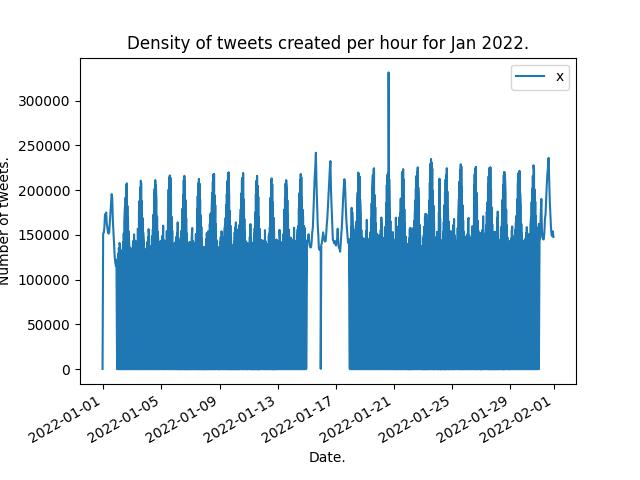
\includegraphics[scale=0.3]{figures/JanAllraw.jpeg}
    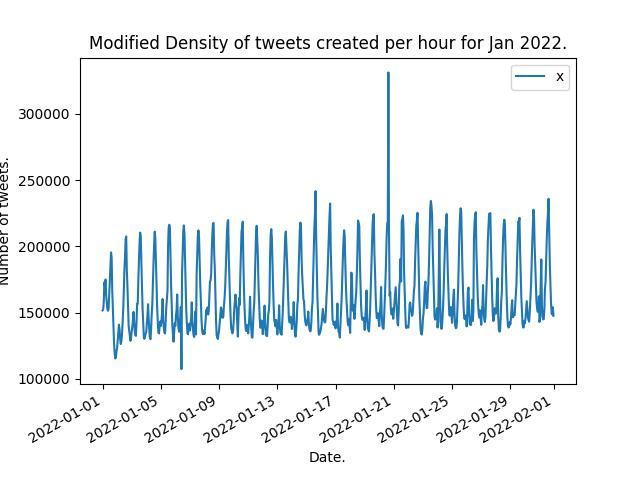
\includegraphics[scale=0.3]{figures/JanAllmod.jpeg}
    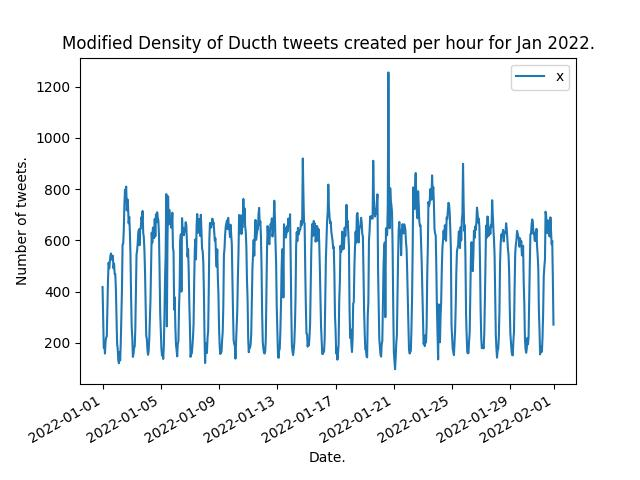
\includegraphics[scale=0.3]{figures/JanNLmod.jpeg}
\end{figure}

Since we are looking at discrete time events, we would like to have a better resolution of
the density of tweets per a time period. We achieve this by selecting again only the
Dutch tweets and then choosing a smaller time bin, in this case of `2min`, while doing so
we also choose a smaller range of data, as we have index the dataframe by a Timestamp data
type, hence we can focus on 14-01-2022. Plotting this we see large fluctuations in the
data points, making the plot hard to read. The readability can be improved by using the
pandas rolling function in alignment of the mean function, the result is a smooth rolling
mean plot of the data.


\begin{figure}[h!]
    \center
    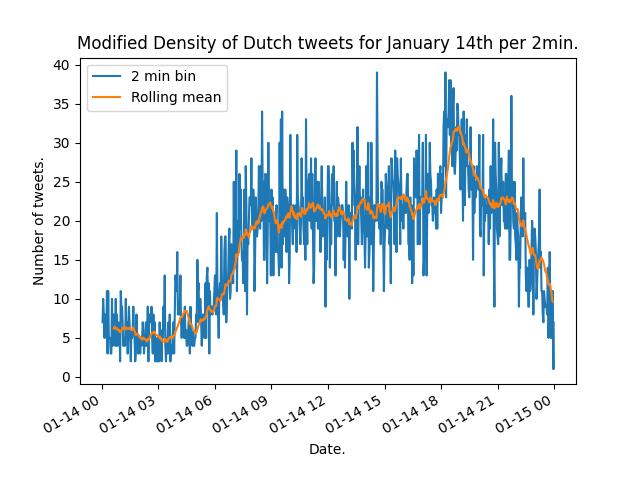
\includegraphics[scale=0.3]{figures/JanNLD14roll.jpeg}
    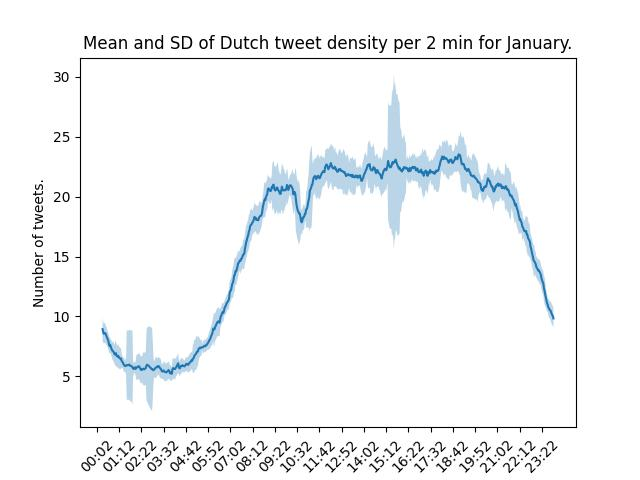
\includegraphics[scale=0.3]{figures/JanNLdayfill.jpeg}
\end{figure}

\section{Conclusion}








\end{document}
